\subsection{Raman coupling Hamiltonian}\label{Raman}
\begin{figure}[htbp]
    \centering
    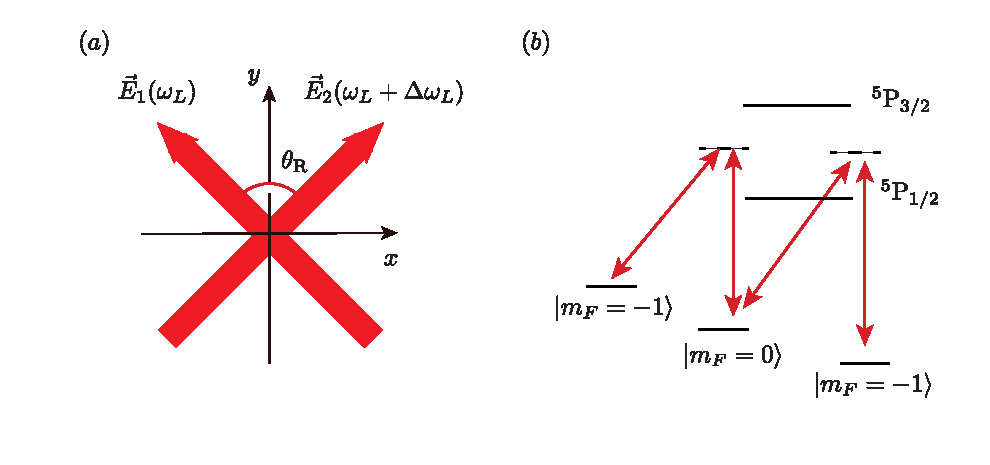
\includegraphics[width=\textwidth]{Chapter3_secs/Raman.pdf}
    \caption{Raman coupling. (a). Two laser beams perpendicular to each other are detuned by $\Delta\omega_L$, they  intersect at the atoms. (b). Hyperfine states coupled by Raman lasers.  }
    \label{fig:Raman}
\end{figure}
Here we derive Raman coupling Hamiltonian and discuss how Raman coupling leads to SOC. Intuitively, SOC generated by Raman coupling can be understood from the momentum transfer in the two-photon process. For example, state $\ket{F=1,m_F=-1}$ absorbs a photon from beam $\Vec{E}_1$ and emits a photon to beam $\Vec{E}_2$, the state transfers to $\ket{F=1,m_F=0}$ and acquires momentum $2k_L$ from the recoil momentum of the two photons. Here $k_L$ is half the difference between the two beams.
\begin{equation}
    k_L = \frac{\sqrt{2}\pi}{\omega_L}.
\end{equation}
Similarly, state $\ket{F=1,m_F=0}$ transfer to $\ket{F=1,m_F=-1}$ and acquires momentum $-2k_L$. State transfer is always accompanied by a momentum transfer of $2k_L$, so the internal states of the atoms are coupled to the momentum states of the atoms. 

Formally, we derive the Raman Hamiltonian in $\ket{F=1}$ manifold. The electric field of the two Raman lasers is
\begin{equation}
    \Vec{E} = \Vec{E}_1e^{i(k_Lx+k_Ly-\omega t)} + \Vec{E}_2e^{i[-k_Lx+k_Ly-(\omega+\Delta\omega_L)t]} + c.c
\end{equation}
Electric dipole interaction Hamiltonian is
\begin{equation}
    \hat{H}_{Dip} = E_e\dyad{e}{e} + E_g\dyad{-1}{-1} - E_g\dyad{1}{1} + \Vec{E}\cdot \Vec{\mu}\left(\dyad{e}{-1} + \dyad{e}{0} + \dyad{e}{1}\right) + c.c
\end{equation}
Expand the wave function in the four state basis,
\begin{equation}
    \psi(t) = a_e(t)\ket{e} + a_{-1}(t)\ket{-1} + a_0(t)\ket{0} + a_1(t)\ket{1},
\end{equation}
First, transform into a rotating frame, 
\begin{equation}
    \Tilde{a}_e = a_ee^{i\omega_Lt}, \Tilde{a}_{-1} = a_{-1}e^{i\Delta\omega_Lt},\Tilde{a}_{1} = a_{1}e^{-i\Delta\omega_Lt} 
\end{equation}
and make rotating wave approximation. Next, due to the large single-photon detuning $\Delta = E_e-\hbar \omega_L$, the excited state $\ket{\Tilde{e}}$ can be adiabatically eliminated ($\frac{d\Tilde{a}_e}{dt} \approx 0$). The effective Hamiltonian of dipole interaction in the $\ket{F=1}$ manifold is
\begin{equation}
\hat{H}_{eff,Dip} = 
\begin{pmatrix}
\hbar\delta & -\hbar\frac{\Omega_1^*\Omega_2}{\Delta}e^{-i2k_Lx} & 0\\
-\hbar\frac{\Omega_1\Omega_2^*}{\Delta}e^{i2k_Lx}  & 0 & -\hbar\frac{\Omega_1^*\Omega_2}{\Delta}e^{-i2k_Lx}\\
0 & -\hbar\frac{\Omega_1\Omega_2^*}{\Delta}e^{i2k_Lx} & -\hbar\delta\\
\end{pmatrix}
 - \hbar\frac{(|\Omega_1|^2 + |\Omega_2|^2)}{\Delta}.
\end{equation}
The last term is the AC stack shift for all the sub states. $\delta = E_g - \Delta\omega_L$ is the two-photon detuning. When quadratic Zeeman shift \ref{zeeman chpt} is considerred, state $\ket{1}$ is far detuned from the other two states and can be eliminated. The two level effective Hamiltonian takes the form
\begin{equation}
    \hat{H}_{eff} = \frac{\hbar^2\hat{k}^2}{2m}\hat{\mathds{1}} + \frac{\delta}{2}\hat{\sigma}_z + \Omega_R\hat{\sigma}_x\cos{2k_Lx} - \Omega_R^*\hat{\sigma}_y\sin{2k_Lx}
\end{equation}
here,
\begin{equation}
    \Omega_R = -\hbar\frac{\Omega_1^*\Omega_2}{\Delta}
\end{equation}
is the effective Raman coupling strength. Finally, by applying a position dependent rotational transformation
\begin{equation}
    e^{\frac{i\hat{\sigma}_z 2k_Lx}{\hbar}},    
\end{equation}
we arrive at the SOC form of the Hamiltonian
\begin{equation}
    \hat{H}_{SOC} =  \frac{\hbar^2\hat{k}^2}{2m}\hat{\mathds{1}} + \Omega_R\hat{\sigma}_z + \frac{\delta}{2}\hat{\sigma}_y + \frac{\hbar^2k_L}{m}\hat{k}_x\hat{\sigma}_y
\end{equation}
which has equal contribution of Rashba and Dresselhaus SOC.
